\section{Model}
From \autoref{app:journal_speaker_test3} and the previous section the models are determined for the lower frequency bands as:
\begin{enumerate}
\item 33 Hz to 66 Hz
\item 66 Hz to 132 Hz
\item 132 Hz to 265 Hz
\item 265 Hz to 530 Hz,
\end{enumerate}
Futhermore a limiter placed from 500 hz and down will be implemented. This limiter will provide limitation if the entire band exceeds an RMS value great enough to introduce 150 watts into the speaker. The 4 other bands will also be subjected to individual limitation based on a worst case model of each band. As stated before the models are based on experiments documented in \autoref{app:journal_speaker_test3}. These models are depicted in \autoref{fig:CombinedModelreport} and shows THD according to the RMS value. The models are created by 2.order polynomial regression of discrete THD value calculated from microphone measurements. Hence the model of band 1 should not be considered valid unless an RMS value of at least 0.25 is present.

\begin{figure}[H]
    \centering
    \tikzsetnextfilename{BandModelCombineReport}
    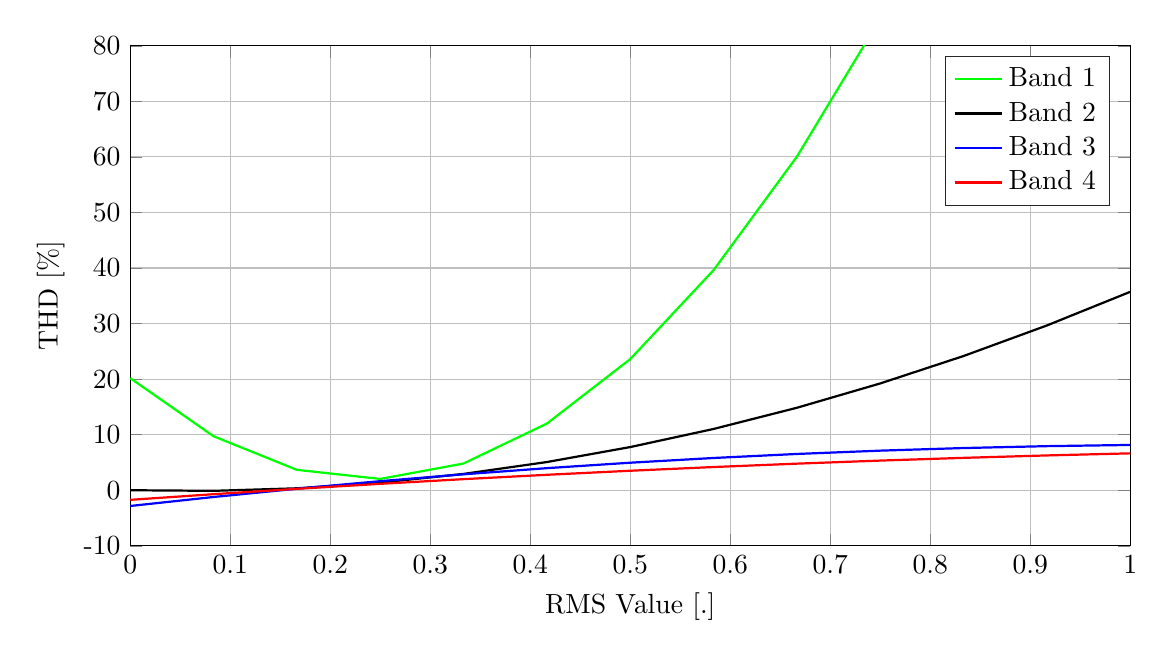
\begin{tikzpicture}

\begin{axis}[%
width=5.0in,
height=2.5in,
at={(0.758in,0.481in)},
scale only axis,
xmin=0,
xmax=1,
xmajorgrids,
ymajorgrids,
xlabel={RMS Value [.]},
ymin=-0.1,
ymax=0.8,
ylabel={THD [\%]},
ytick={-0.1, 0, 0.1,  0.2,  0.3, 0.4, 0.5, 0.6, 0.7, 0.8},
yticklabels={-10,0,10,20,30,40,50,60,70,80},
axis background/.style={fill=white},
legend style={legend cell align=left,align=left,draw=white!15!black}
%every axis legend/.code={\let\addlegendentry\relax}
]
\addplot [color=green,solid,thick]
  table[row sep=crcr]{%
0	0.2018\\
0.0833333333333333	0.0971958333333334\\
0.166666666666667	0.0367166666666667\\
0.25	0.0203625\\
0.333333333333333	0.0481333333333334\\
0.416666666666667	0.120029166666667\\
0.5	0.23605\\
0.583333333333333	0.396195833333334\\
0.666666666666667	0.600466666666667\\
0.75	0.8488625\\
0.833333333333333	1.14138333333333\\
0.916666666666667	1.47802916666667\\
1	1.8588\\
};
\addlegendentry{Band 1};


\addplot [color=black,solid,thick]
  table[row sep=crcr]{%
0	0\\
0.0833333333333333	-0.00105625\\
0.166666666666667	0.00349166666666667\\
0.25	0.01364375\\
0.333333333333333	0.0294\\
0.416666666666667	0.0507604166666667\\
0.5	0.077725\\
0.583333333333333	0.11029375\\
0.666666666666667	0.148466666666667\\
0.75	0.19224375\\
0.833333333333333	0.241625\\
0.916666666666667	0.296610416666667\\
1	0.3572\\
};
\addlegendentry{Band 2};

\addplot [color=blue,solid,thick]
  table[row sep=crcr]{%
0	-0.02834\\
0.0833333333333333	-0.0121695138888889\\
0.166666666666667	0.00272527777777777\\
0.25	0.016344375\\
0.333333333333333	0.0286877777777778\\
0.416666666666667	0.0397554861111111\\
0.5	0.0495475\\
0.583333333333333	0.0580638194444444\\
0.666666666666667	0.0653044444444444\\
0.75	0.071269375\\
0.833333333333333	0.0759586111111111\\
0.916666666666667	0.0793721527777778\\
1	0.08151\\
};
\addlegendentry{Band 3};

\addplot [color=red,solid,thick]
  table[row sep=crcr]{%
0	-0.01729\\
0.0833333333333333	-0.00709902777777778\\
0.166666666666667	0.00250722222222222\\
0.25	0.01152875\\
0.333333333333333	0.0199655555555556\\
0.416666666666667	0.0278176388888889\\
0.5	0.035085\\
0.583333333333333	0.0417676388888889\\
0.666666666666667	0.0478655555555556\\
0.75	0.05337875\\
0.833333333333333	0.0583072222222222\\
0.916666666666667	0.0626509722222222\\
1	0.06641\\
};
\addlegendentry{Band 4};

\end{axis}
\end{tikzpicture}
    \caption{4 Interpolated model describing the worst case THD in each band. Further described in \autoref{app:journal_speaker_test3}}
    \label{fig:CombinedModelreport}
\end{figure}

From \autoref{fig:CombinedModelreport} it should be noted that the models only describe the THD from single tone test. Compared with regular music which contains many single tones combined. However from the models it can be concluded that the lower frequency bands should be limited more than the higher frequency bands. It gives means to choose a lower threshold for the first band than for the third band and up. This correlates with the first band is subjected to the resonance frequency of the driver. Already in the second band the THD much more linear and can cope with a higher threshold

\vspace{2mm}
Since the need for limitations in the third and fourth band is not as critical compared as with the first and second band, it would be logical to choose a THD value and find the respective threshold for band 1 and 2. Where as the third and fourth band should be made equal to the limiter covering the entire 500 Hz spectrum. The goal of this project is however to prevent a possible hit against the backplate and since this is documented to occur at 150 watt the parameters will solely be based on the 150 watt threshold. 